\documentclass[11pt,a0paper]{article}
\usepackage{tikz-qtree}
\usepackage{tikz}
\usepackage[landscape]{geometry}
\begin{document}
\pagestyle{empty}
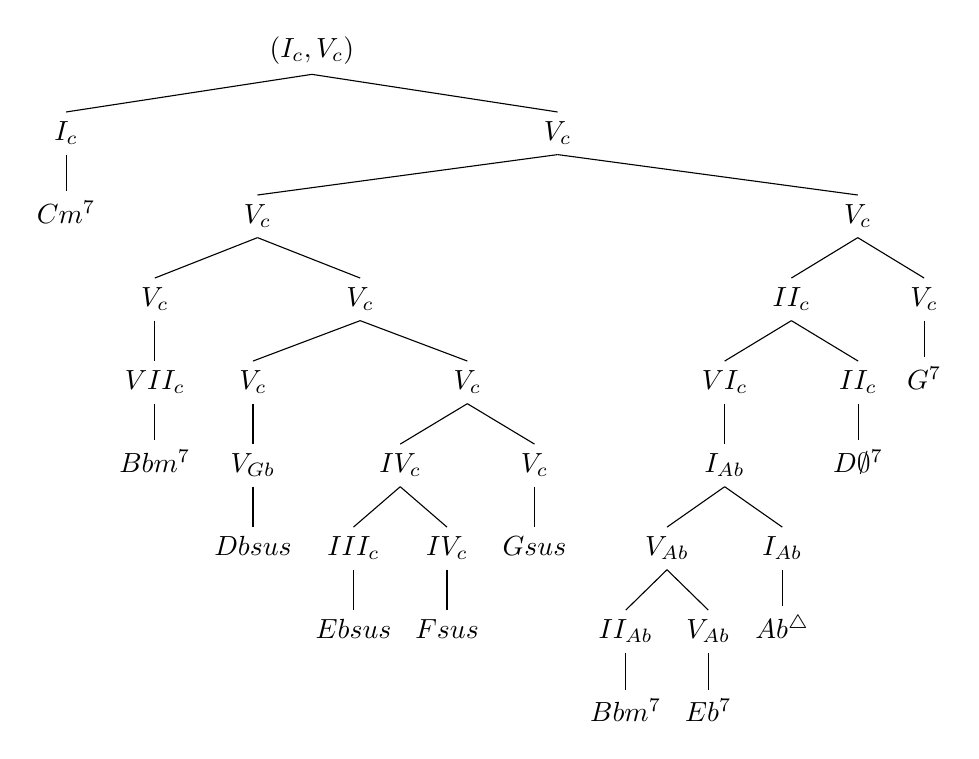
\begin{tikzpicture}[level distance=30pt]
\tikzset{frontier/.style={distance from root=8*30pt}}
    \Tree  [.{$(I_{c},V_{c})$} [.{$I_{c}$} [.{$Cm^7$} ]  ]  [.{$V_{c}$} [.{$V_{c}$} [.{$V_{c}$} [.{$VII_{c}$} [.{$Bbm^7$} ]  ]  ]  [.{$V_{c}$} [.{$V_{c}$} [.{$V_{Gb}$} [.{$Dbsus$} ]  ]  ]  [.{$V_{c}$} [.{$IV_{c}$} [.{$III_{c}$} [.{$Ebsus$} ]  ]  [.{$IV_{c}$} [.{$Fsus$} ]  ]  ]  [.{$V_{c}$} [.{$Gsus$} ]  ]  ]  ]  ]  [.{$V_{c}$} [.{$II_{c}$} [.{$VI_{c}$} [.{$I_{Ab}$} [.{$V_{Ab}$} [.{$II_{Ab}$} [.{$Bbm^7$} ]  ]  [.{$V_{Ab}$} [.{$Eb^7$} ]  ]  ]  [.{$I_{Ab}$} [.{$Ab^\triangle$} ]  ]  ]  ]  [.{$II_{c}$} [.{$D\emptyset^7$} ]  ]  ]  [.{$V_{c}$} [.{$G^7$} ]  ]  ]  ]  ] 
\end{tikzpicture}
\end{document}
